%!TEX root = head-full.tex

\section{Metropolis-Hastings} \label{sec:metropolis_hastings}
Metropolis Hastings(MH) Algorithm

\subsection{Algorithm\protect\footnote{Available at \protect\url{https://github.com/lzhbrian/MCMC/blob/master/metropolis_hastings/metropolis_hasting.R} in Matlab}}

\subsubsection{Detailed Balance Condition}

\subsubsection{General Case}

\subsubsection{Symmetric Case}




\subsection{Sampling Results}
In our work, we use an example of a bivariate Normal distribution, with
$$ \mu = \left( \begin{array}{ccc}
5 \\
10 \end{array} \right), 
\Sigma = \left( \begin{array}{ccc}
1 & 1\\
1 & 4\end{array} \right)$$

By theoretical computation, we can easily compute the the pearson correlation between the two dimensional value is 0.5.
$$ \rho = 0.5 $$

We then generate 10,000 samples using the MH algorithm, setting the standard deviation of proposal to 3.0. We can see from the result (Figure~\ref{fig:sample_result}) that we have derived 10,000 sampled points with pearson correlation = 0.5, which matches the theoretical value.

\begin{figure}[t]
\vspace{-0.5in}
  	\centering
  	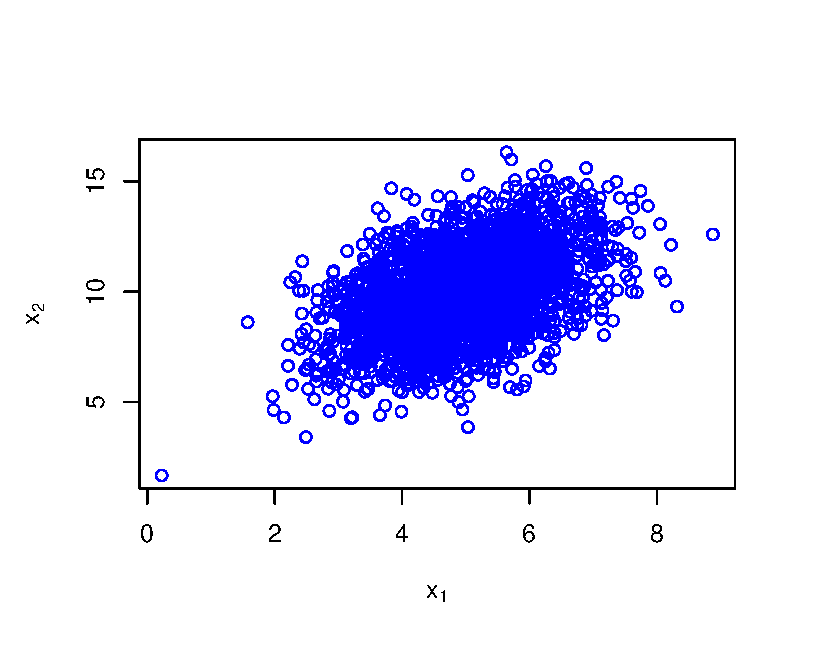
\includegraphics[width=0.4\textwidth]{figure/sample_result.eps}
\vspace{-0.2in}
	\caption{Sampling result of 10,000 points \protect\\ correlation = 0.500873 , set sd.T = 3.0}
	\label{fig:sample_result}
\end{figure}


\subsection{Performance Analysis}
MH algorithm is an effective MCMC method for many diverse problems. However, its efficiency depends crucially on the selection of the proposal density. With the proposal jump size being small, the accepting rate would be very low and eventually stick to only one point(eg. the initial point); When the proposal jump size is too big, the accepting rate would be too high. 

Roberts et al. have shown in previous work\cite{roberts1997weak} that the optimal accepting rate of the MH algorithm should approximately be at 0.234 for the case of an N-dimensional Gaussian target distribution. We test the accepting rates in different proposal jump size(Figure~\ref{fig:acc_sdt}) and find that the optimal value should be at appoximately 3.0 to acquire a model with accepting rate being close to 0.234.

\begin{figure}[t]
\vspace{-0.5in}
  	\centering
  	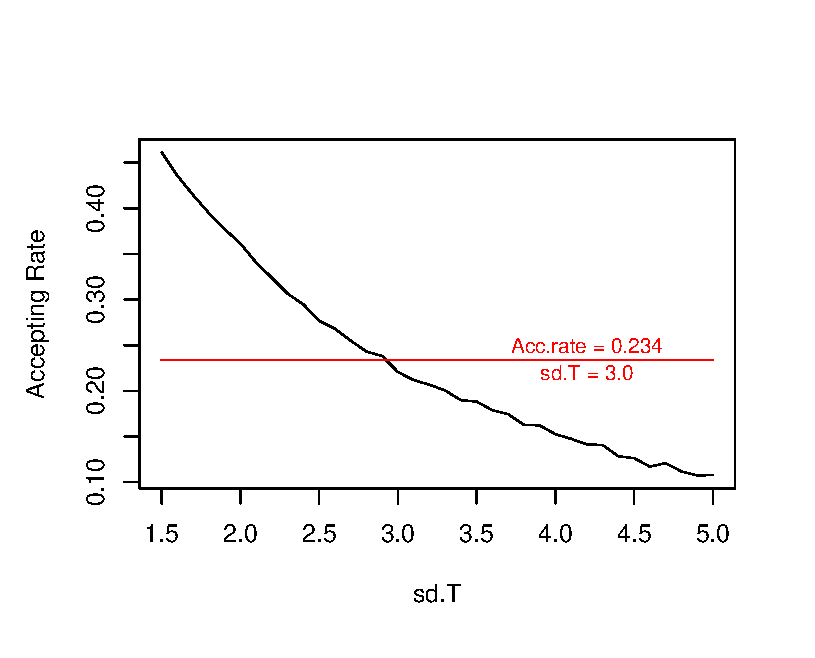
\includegraphics[width=0.4\textwidth]{figure/acc_sdt.eps}
\vspace{-0.2in}
	\caption{Accepting rate on different proposal jump size.}
	\label{fig:acc_sdt}
\end{figure}

\subsection{Gibbs Sampling}
For a high dimensional condition, because of the limit of accepting rate, the efficiency of MH algorithm is not satisfying, so many would switch to Gibbs Sampling Algorithm.

Gibbs Sampling is a special case of Metropolis Hastings Algorithm, by letting the accepting rate = 1, we will get a Gibbs Sampler. As the length \& time limit, we will not specify more here.






